\chapter[Soluciones individuales de series de Fourier]{Soluciones individuales de series de Fourier}
\label{cp:user-guide}

{
\parindent0pt

En este apartado se presentan las soluciones individuales de cada estudiante, desarrolladas a partir de las funciones propuestas por el profesor de la materia de Cómputo Paralelo.El objetivo principal de esta fase fue llevar a cabo el cálculo de la serie de Fourier correspondiente a cada función asignada, aplicando los métodos matemáticos adecuados para la obtención de los coeficientes y la expansión de la función en términos de senos y cosenos.
\vspace{10pt}

Cada integrante del equipo realizó los cálculos de manera independiente, asegurando un desarrollo detallado y estructurado de los coeficientes de Fourier. Para ello, se siguió el procedimiento estándar de integración para la obtención de los coeficientes \(a_0\), \(a_n\) y \(b_n\), que determinan la representación trigonométrica de la función en términos de series de Fourier.
\newpage
% \begin{verbatim}
% 00-Abstract.tex
% 01-Introduction.tex
% 02-User-Guide.tex
% ...
% \end{verbatim}
%---------------------------------------- Ilse

\section{Función resuelta por Castro Paez Ilse Yazbeth}
En este siguiente apartado, se presentan los cálculos para de la serie de Fourier de la función \(f(x)=9-3x-x^2\), correrpondientes a la figura \ref{fig:figure-ilse-01}, donde se muestran detalladamente el desarrollo hasta obtener el resultado. 

\begin{figure}[H]
    \centering
    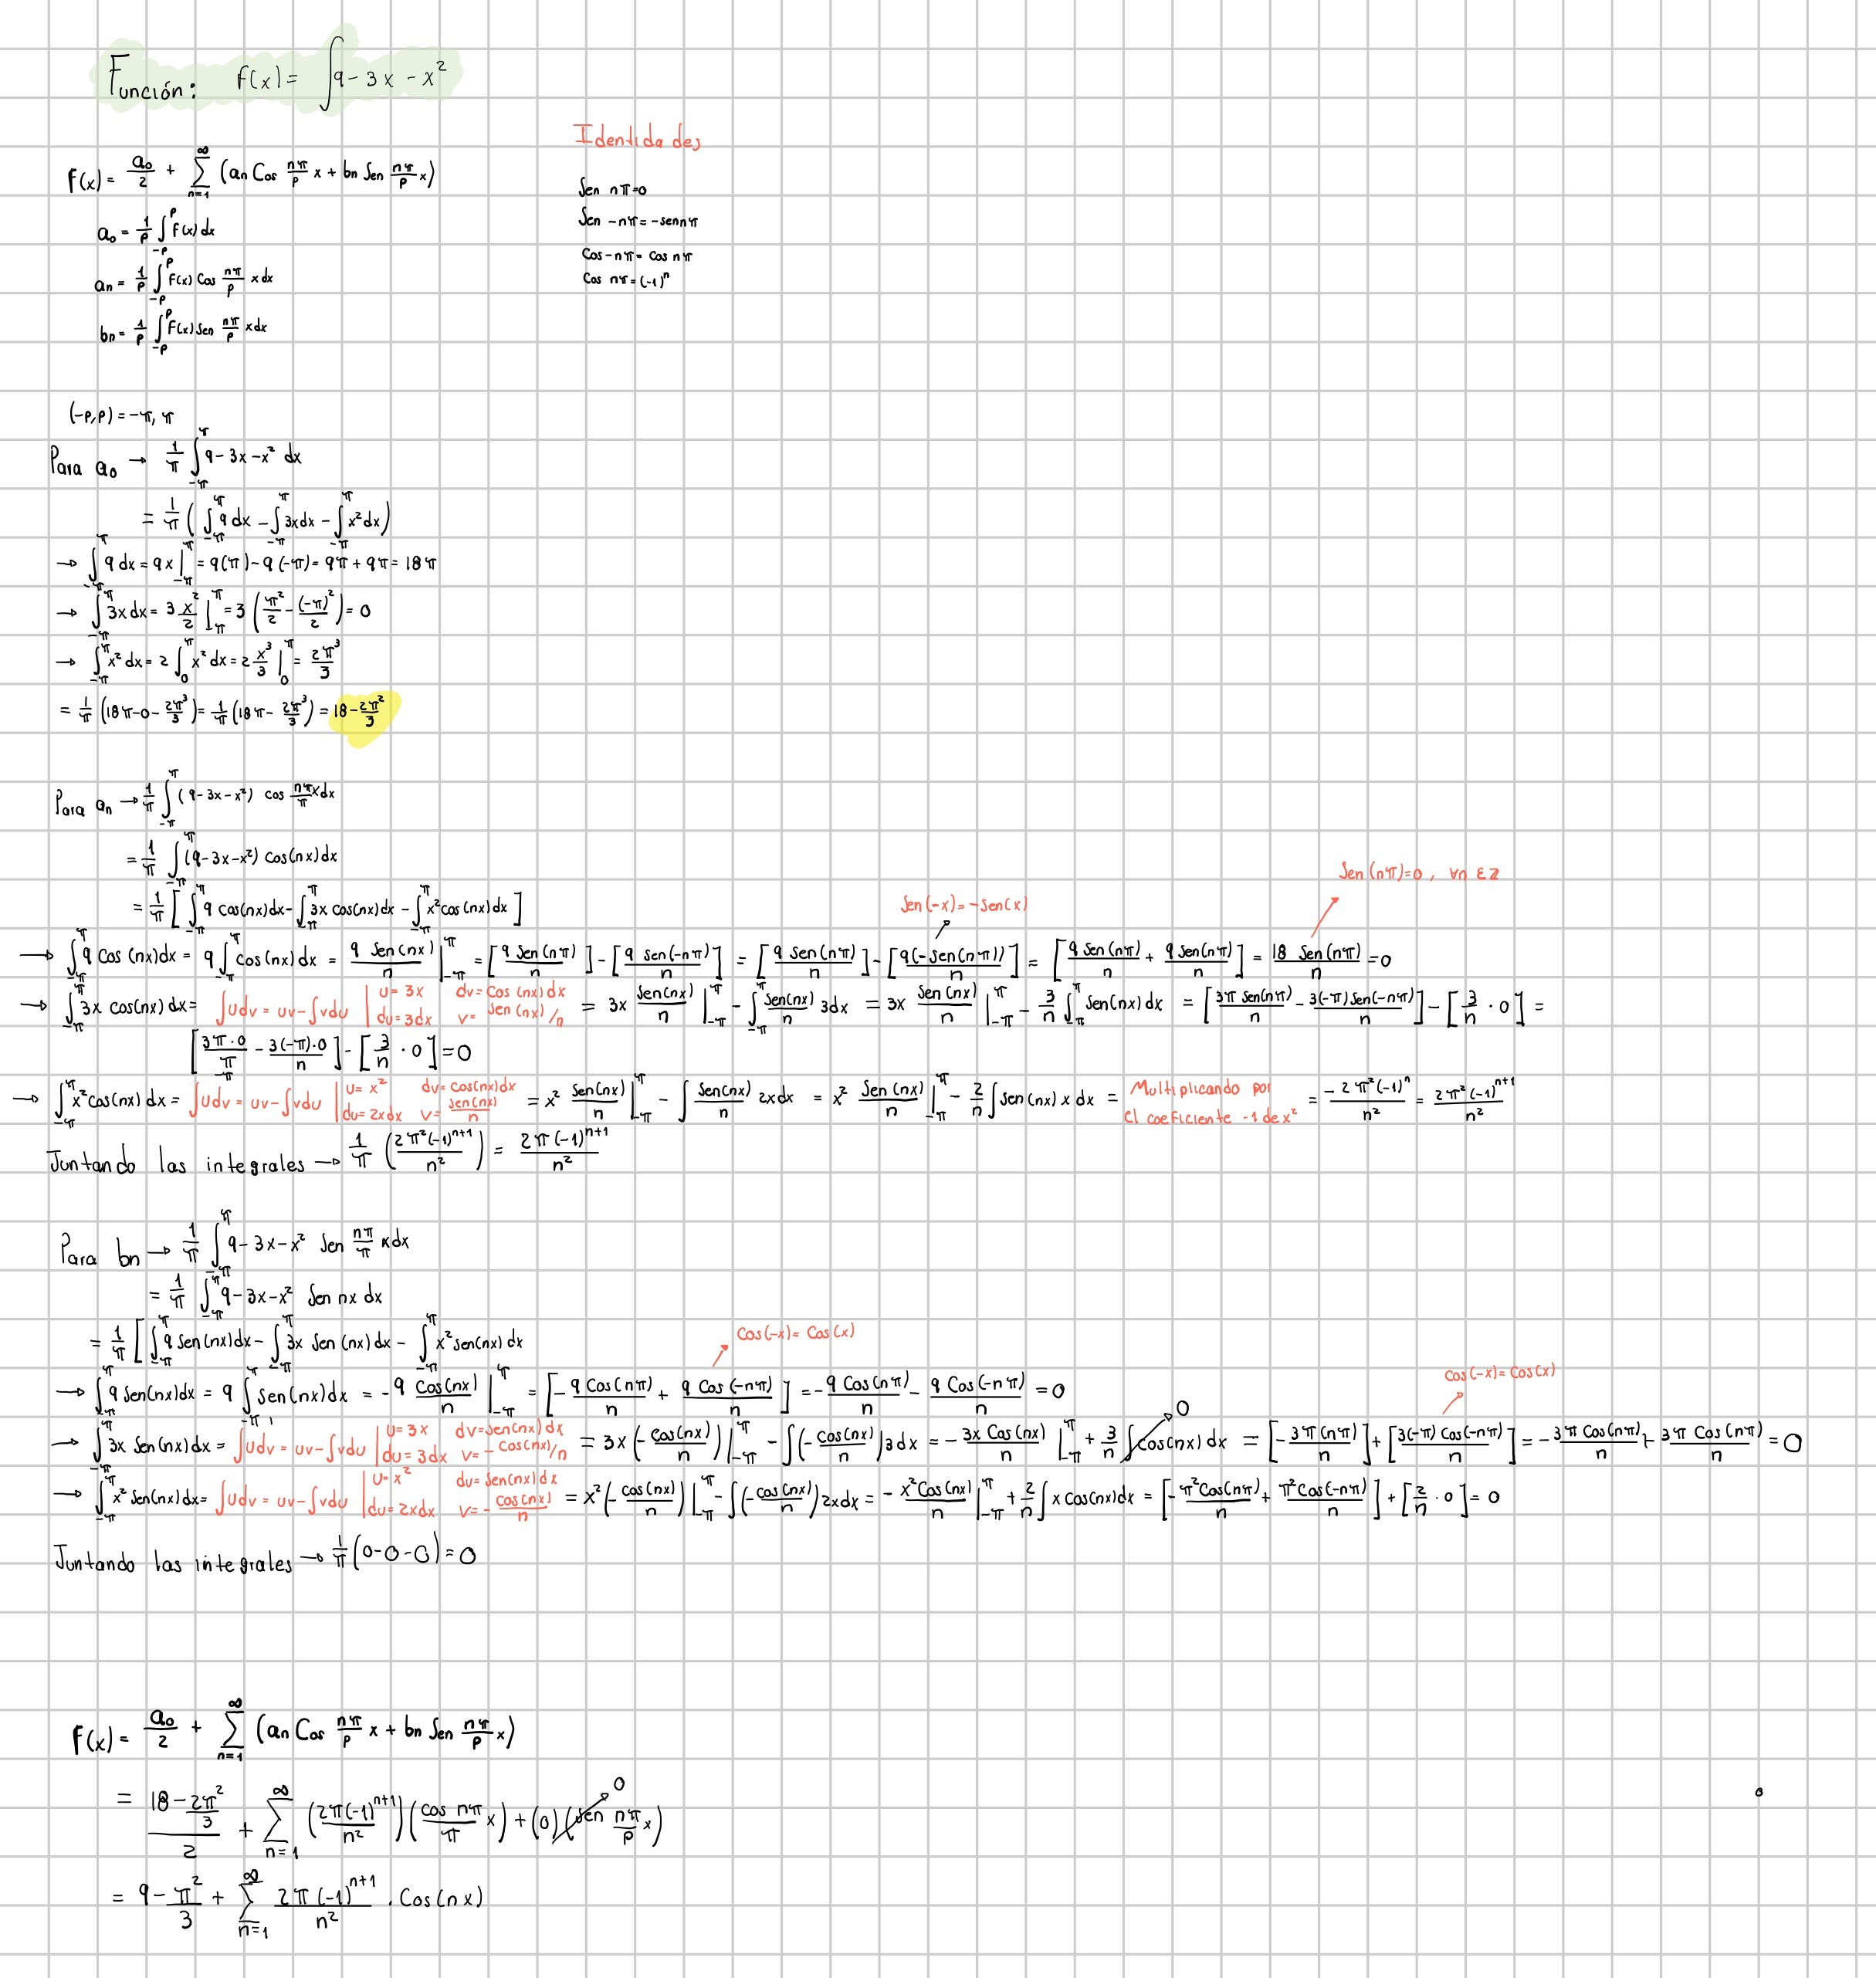
\includegraphics[width=\linewidth]{Figures/fourierIlse/fourierIlse.jpg}
    \caption[Cálculo de la función \(f(x)=9-3x-x^2\)]{Cálculo de la función \(f(x)=9-3x-x^2\), resuelto por Castro Paez Ilse Yazbeth}
    \label{fig:figure-ilse-01}
\end{figure}



%---------------------------------------- Daniel
\newpage
\section{Función resuelta por Catonga Tecla Daniel Isaí}
En el siguiente apartado, se presentan los cálculos para la obtención de los coeficientes de Fourier de la función asignada, \(f(x)=6-2x\), correspondientes a las figuras \ref{fig:figure-daniel-01} hasta \ref{fig:figure-daniel-04}. Se detallan las ecuaciones utilizadas y el procedimiento matemático seguido para su determinación.

\begin{figure}[H]
    \centering
    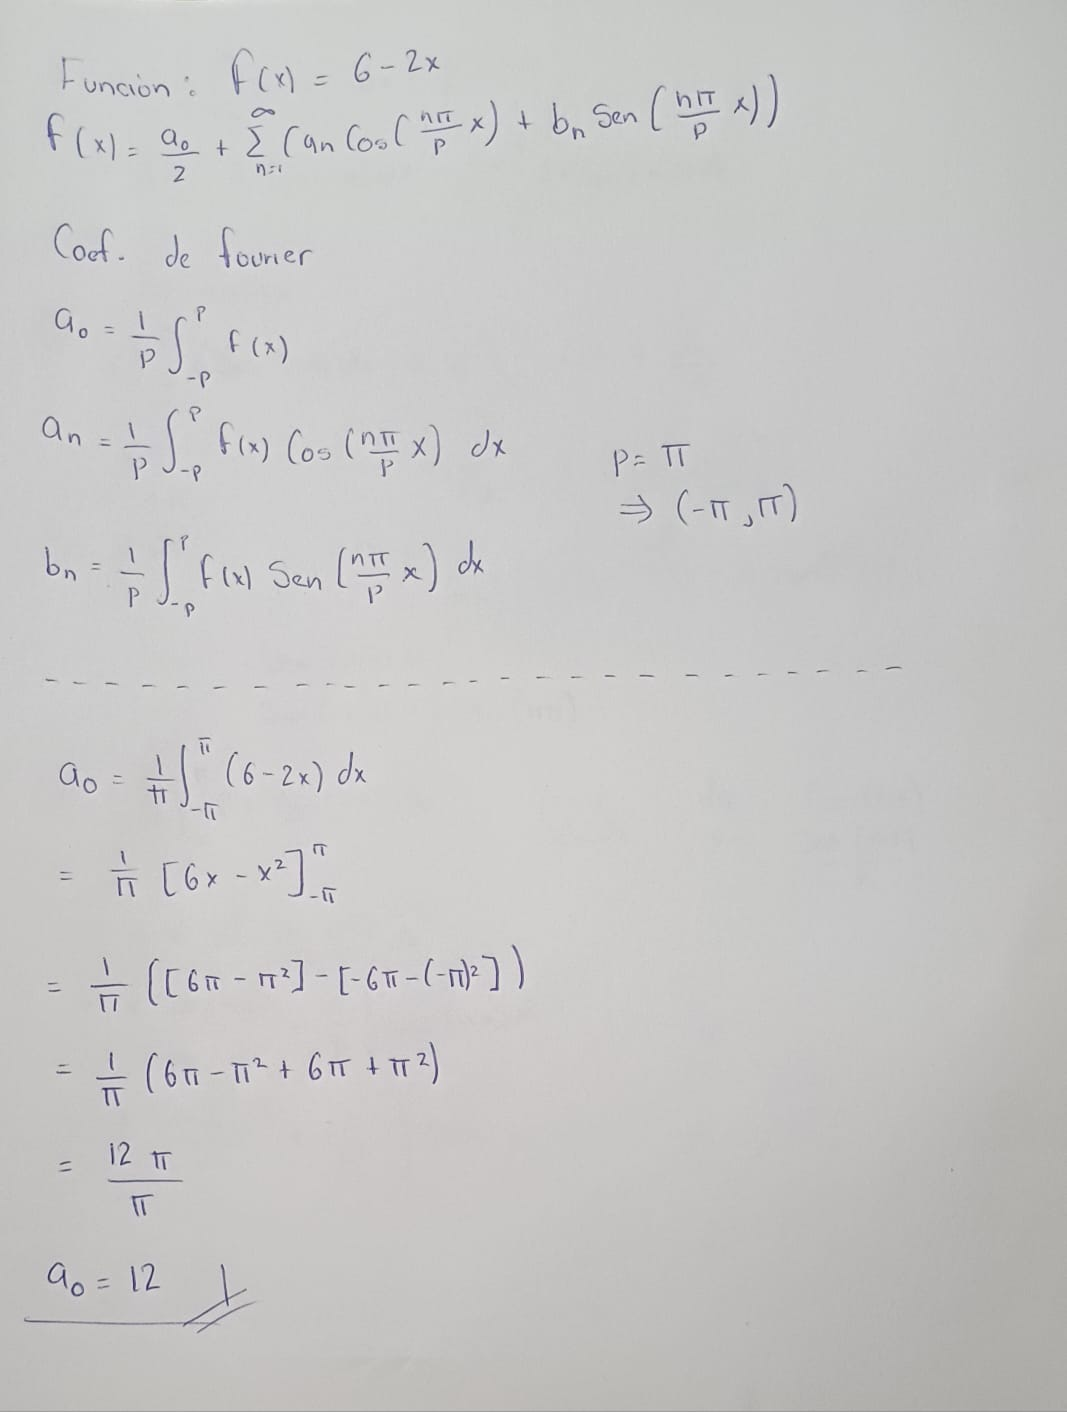
\includegraphics[width=\linewidth]{Figures/fourierDaniel/fourierDaniel1.jpg}
    \caption[Cálculo de \(a_0\) para \(f(x)=6-2x\)]{Cálculo de \(a_0\) para \(f(x)=6-2x\), resuelto por Catonga Tecla Daniel Isaí}
    \label{fig:figure-daniel-01}
\end{figure}

\begin{figure}[H]
    \centering
    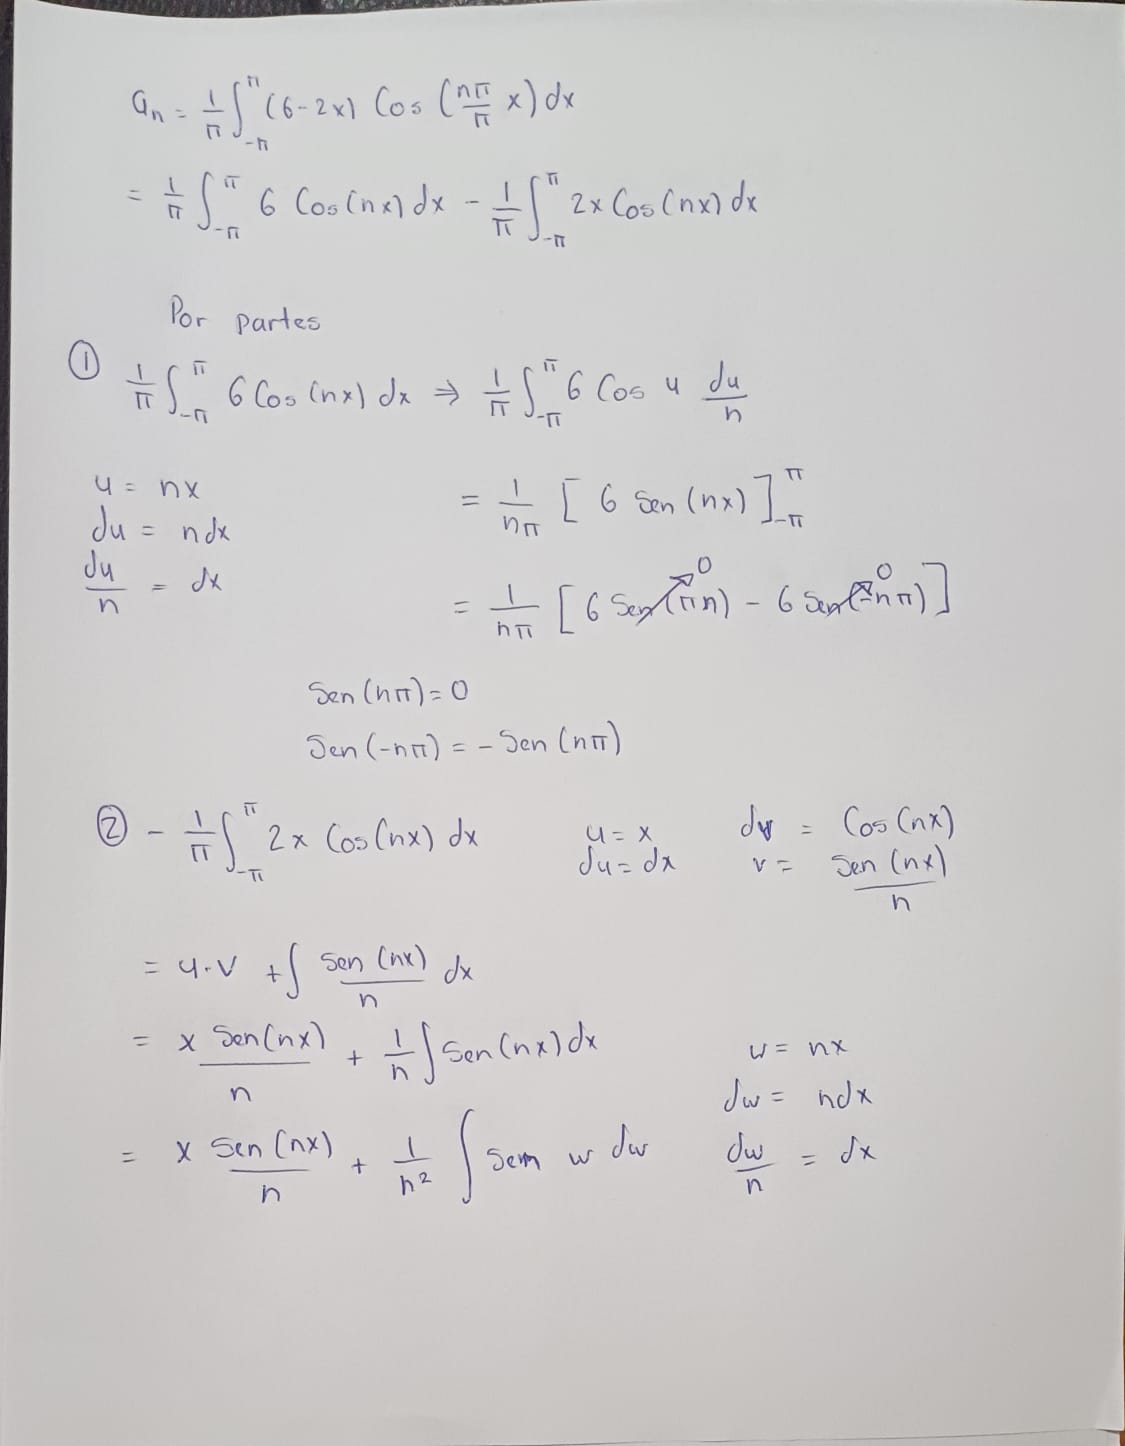
\includegraphics[width=\linewidth]{Figures/fourierDaniel/fourierDaniel2.jpg}
    \caption[Cálculo parcial de \(a_n\) para \(f(x) = 6 - 2x\)]{Desarrollo parcial del cálculo de los coeficientes \(a_n\) para la función \(f(x) = 6 - 2x\), resuelto por Catonga Tecla Daniel Isaí. El resultado final aún no se muestra.}
    \label{fig:figure-daniel-02}
\end{figure}

\begin{figure}[H]
    \centering
    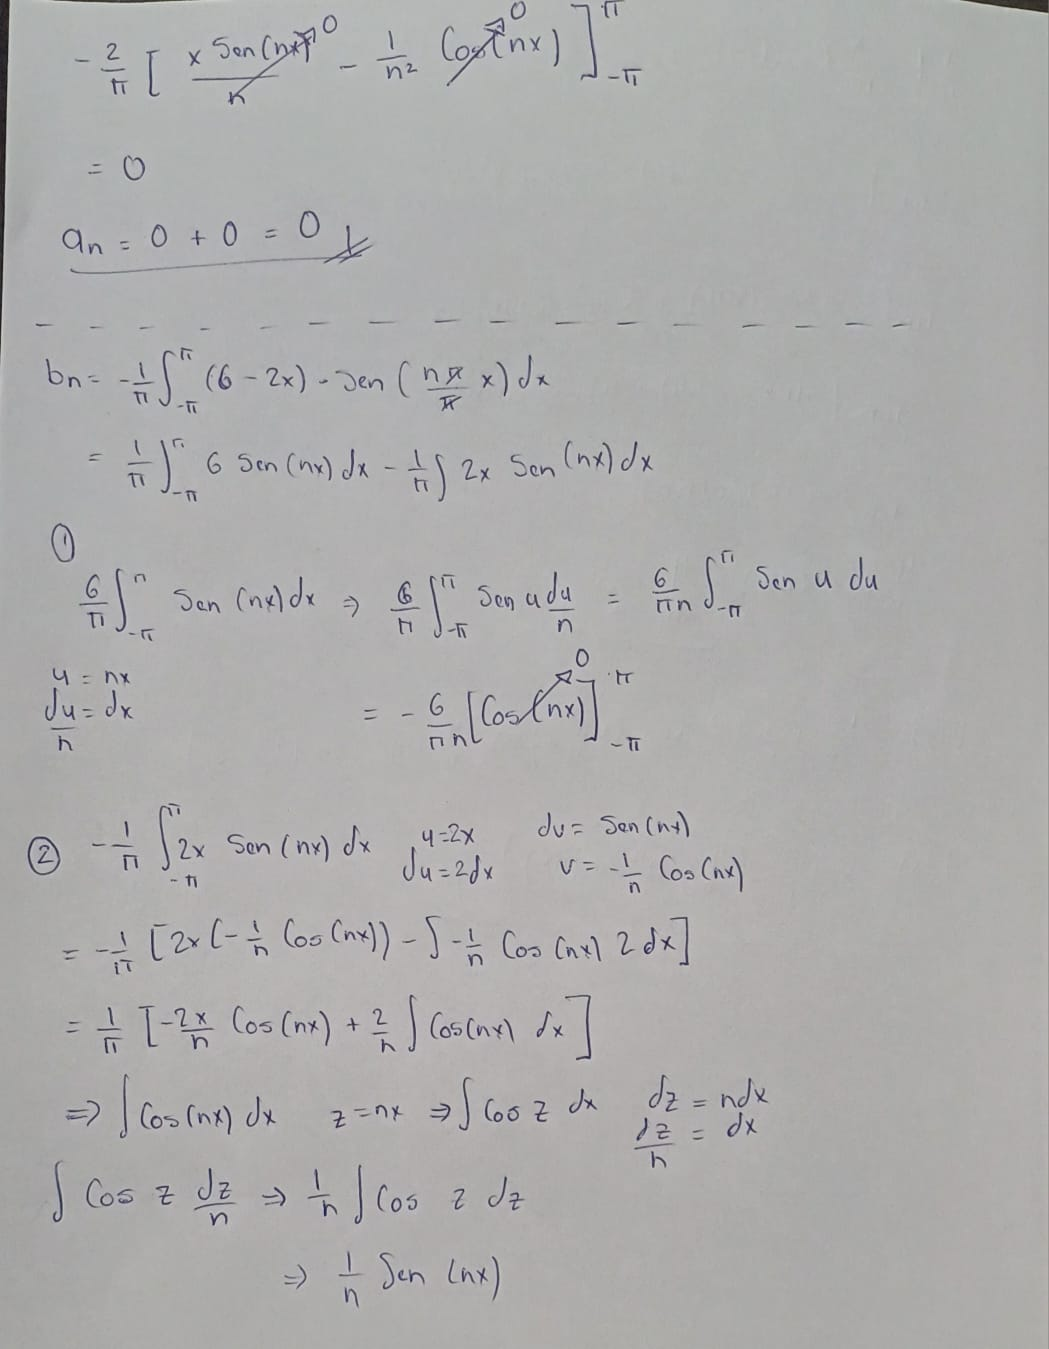
\includegraphics[width=\linewidth]{Figures/fourierDaniel/fourierDaniel3.jpg}
    \caption[Cálculo de \(a_n\) y desarrollo de \(b_n\) para \(f(x) = 6 - 2x\)]{Cálculo de \(a_n\) y desarrollo parcial de \(b_n\) para la función \(f(x) = 6 - 2x\), resuelto por Catonga Tecla Daniel Isaí.}
    \label{fig:figure-daniel-03}
\end{figure}

\begin{figure}[H]
    \centering
    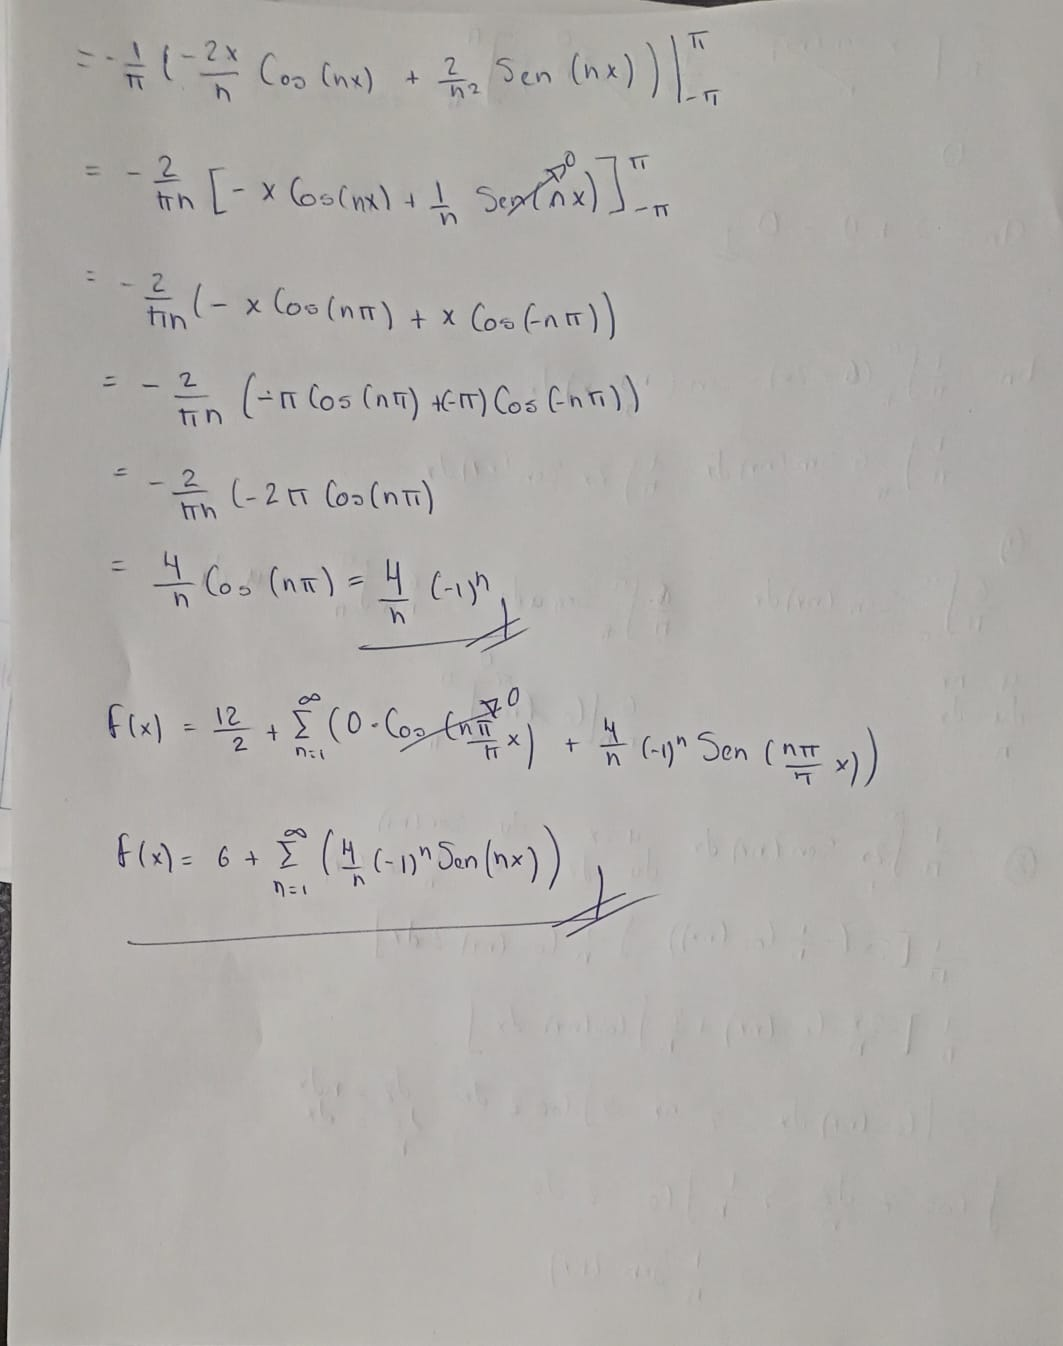
\includegraphics[width=\linewidth]{Figures/fourierDaniel/fourierDaniel4.jpg}
    \caption[Cálculo de \(b_n\) para \(f(x) = 6 - 2x\)]{Cálculo de \(b_n\) para la función \(f(x) = 6 - 2x\), mostrando la función reconstruida a partir de los coeficientes, resuelto por Catonga Tecla Daniel Isaí.}
    \label{fig:figure-daniel-04}
\end{figure}


%-------------------------------------------- Hariel
\newpage
\section{Función resuelta por Padilla Sanchez Hariel }
     En esta sección, se expone el procedimiento matemático para determinar los coeficientes de Fourier de la función \(f(x)=6-4x\). Se inicia con la ecuación general de la serie de Fourier y se procede al cálculo del coeficiente \(a_0\) como se muestra en la figura \ref{fig:figure-hariel-01},Para la obtención de \(a_n\), se emplea integración por partes, evidenciando la cancelación de ciertos términos. Se incluyen además observaciones sobre las propiedades trigonométricas utilizadas en el análisis.

%figura de a0 y an de Hariel 
    \begin{figure}[H]
        \centering
        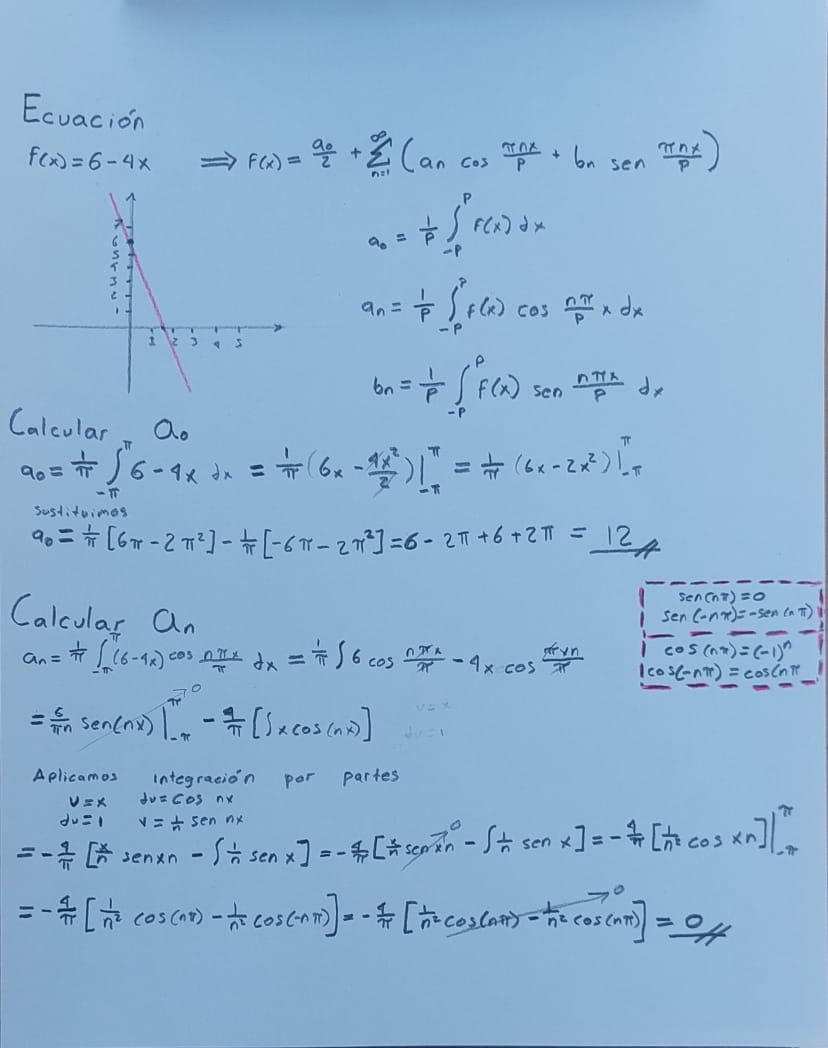
\includegraphics[width=\linewidth]{Figures/fourierHariel/fase1/funcion 1.jpg}
        \caption[Cálculo de \(a_0\) y \(a_n\) para \(f(x) = 6 - 4x\)]{Cálculo de \(a_0\) y \(a_n\) para la función \(f(x) = 6 - 4x\), resuelto por Padilla Sánchez Hariel.}
        \label{fig:figure-hariel-01}
    \end{figure}

    En el siguiente apartado, se presentan los cálculos para la obtención del coeficiente \(b_n\) de la serie de Fourier de la función \(f(x)=6-4x\). Se muestra el desarrollo de la integral correspondiente y la aplicación del método de integración por partes para resolver términos específicos como se muestra en la figura \ref{fig:figure-hariel-02}. Finalmente, se obtiene una expresión general para \(b_n\), la cual se utilizará en la reconstrucción de la función periódica.

%Figura de bn de Hariel
    \begin{figure}[H]
        \centering
        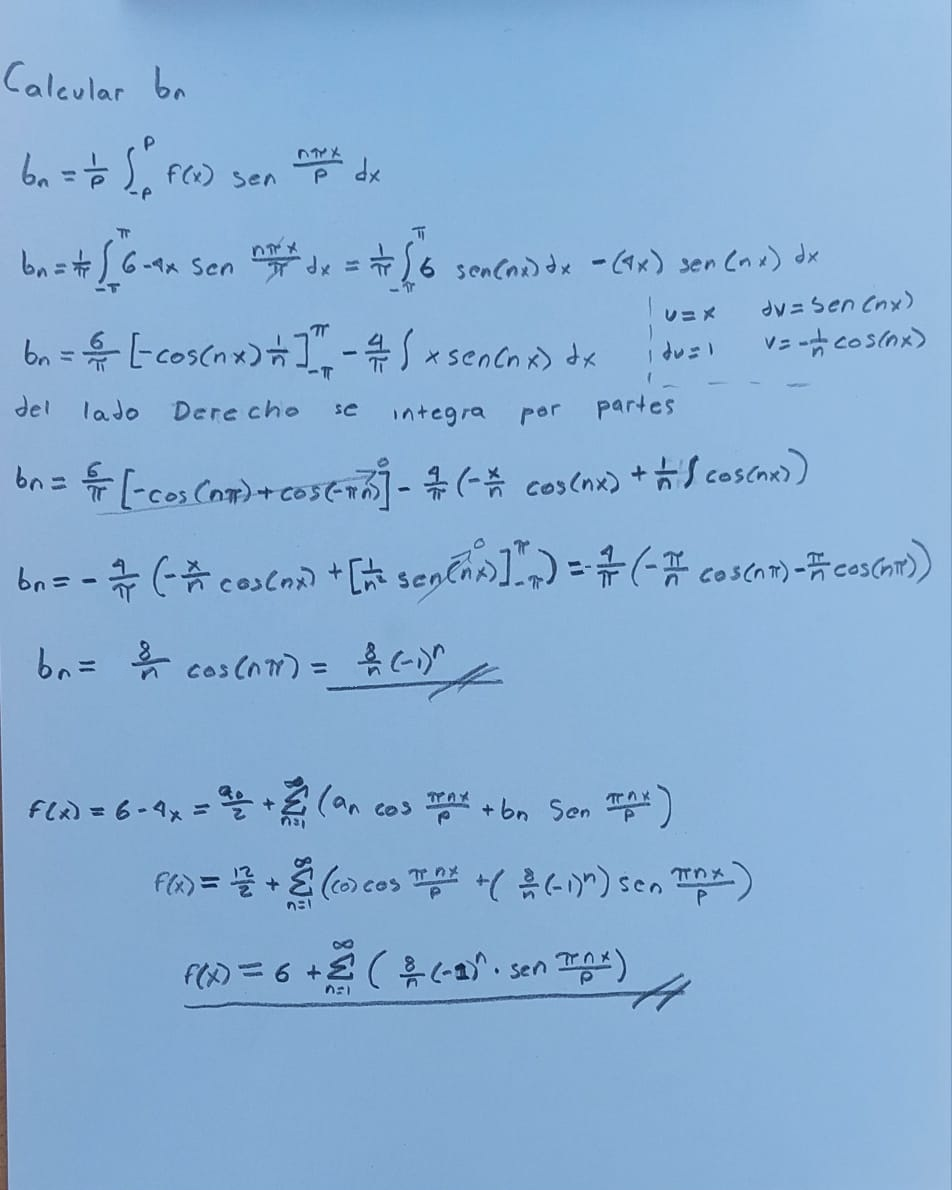
\includegraphics[width=\linewidth]{Figures/fourierHariel/fase1/funcion 2.jpg}
        \caption[Cálculo de \(b_n\) para \(f(x) = 6 - 4x\)]{Cálculo de \(b_n\) para la función \(f(x) = 6 - 4x\), resuelto por Padilla Sánchez Hariel.}
        \label{fig:figure-hariel-02}
    \end{figure}

%-------------------------------------------- Manuel
\section{Función resuelta por Olguin Castillo Víctor Manuel }
    A continuacion se calculan los coeficientes de Fourier asociados a la función \(f(x)=x^2-3x-3\) . 

%figura de a0
    \begin{figure}[H]
        \centering
        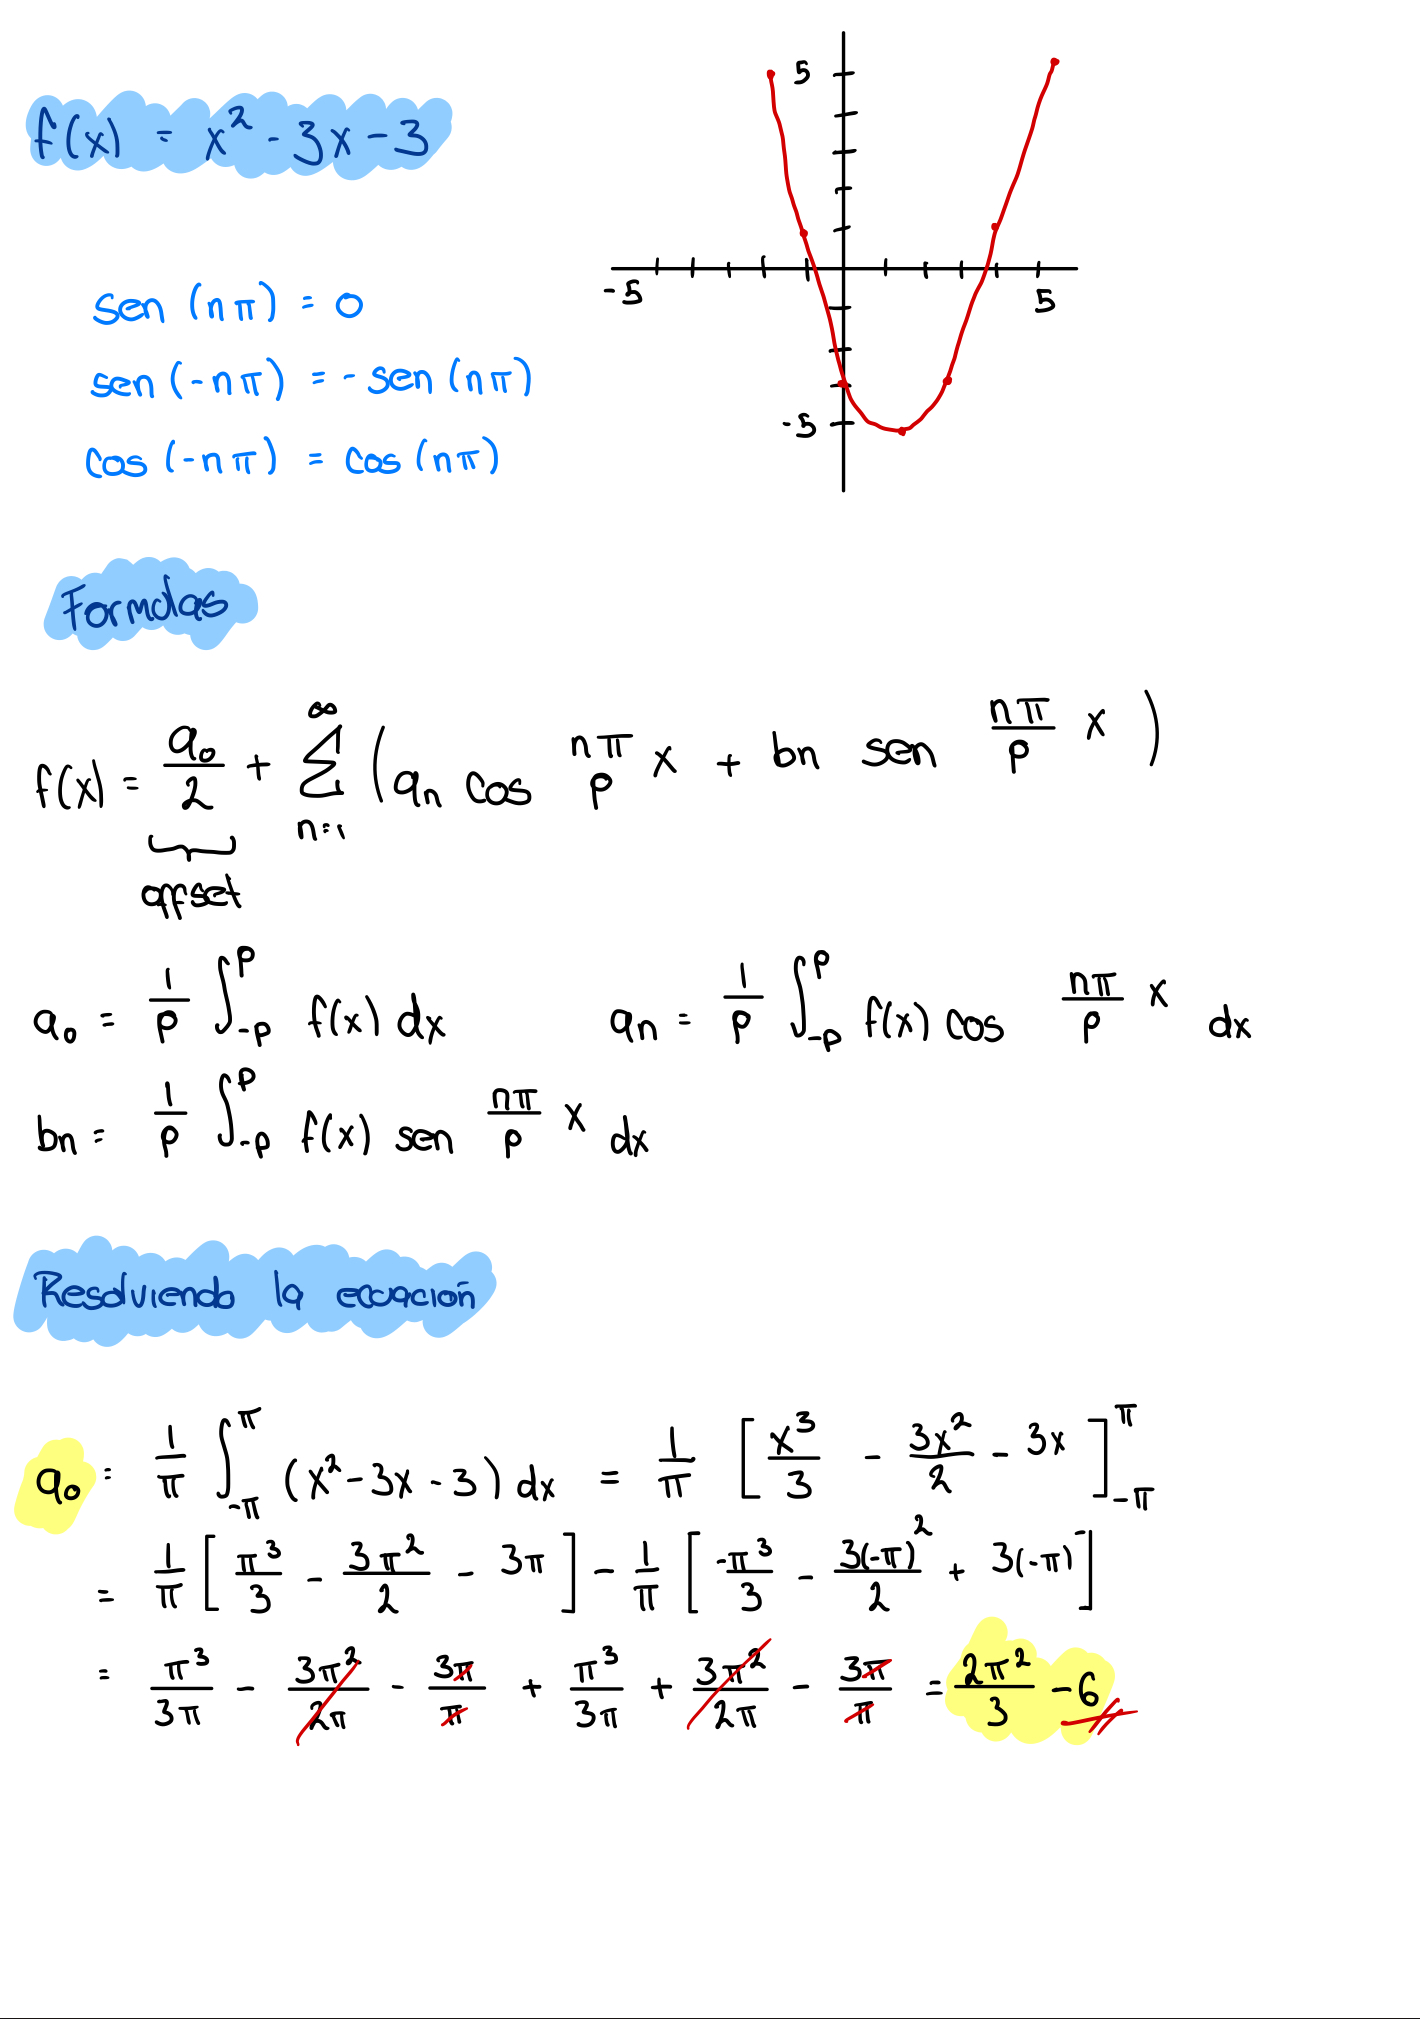
\includegraphics[width=\linewidth]{Figures/fourierManuel/a0.jpeg}
        \caption[Cálculo de \(a_0\)]{Cálculo de \(a_0\), resuelto por Olguin Castillo.}
        \label{fig:figure-manuel-01}
    \end{figure}

%figura de a0
    \begin{figure}[H]
        \centering
        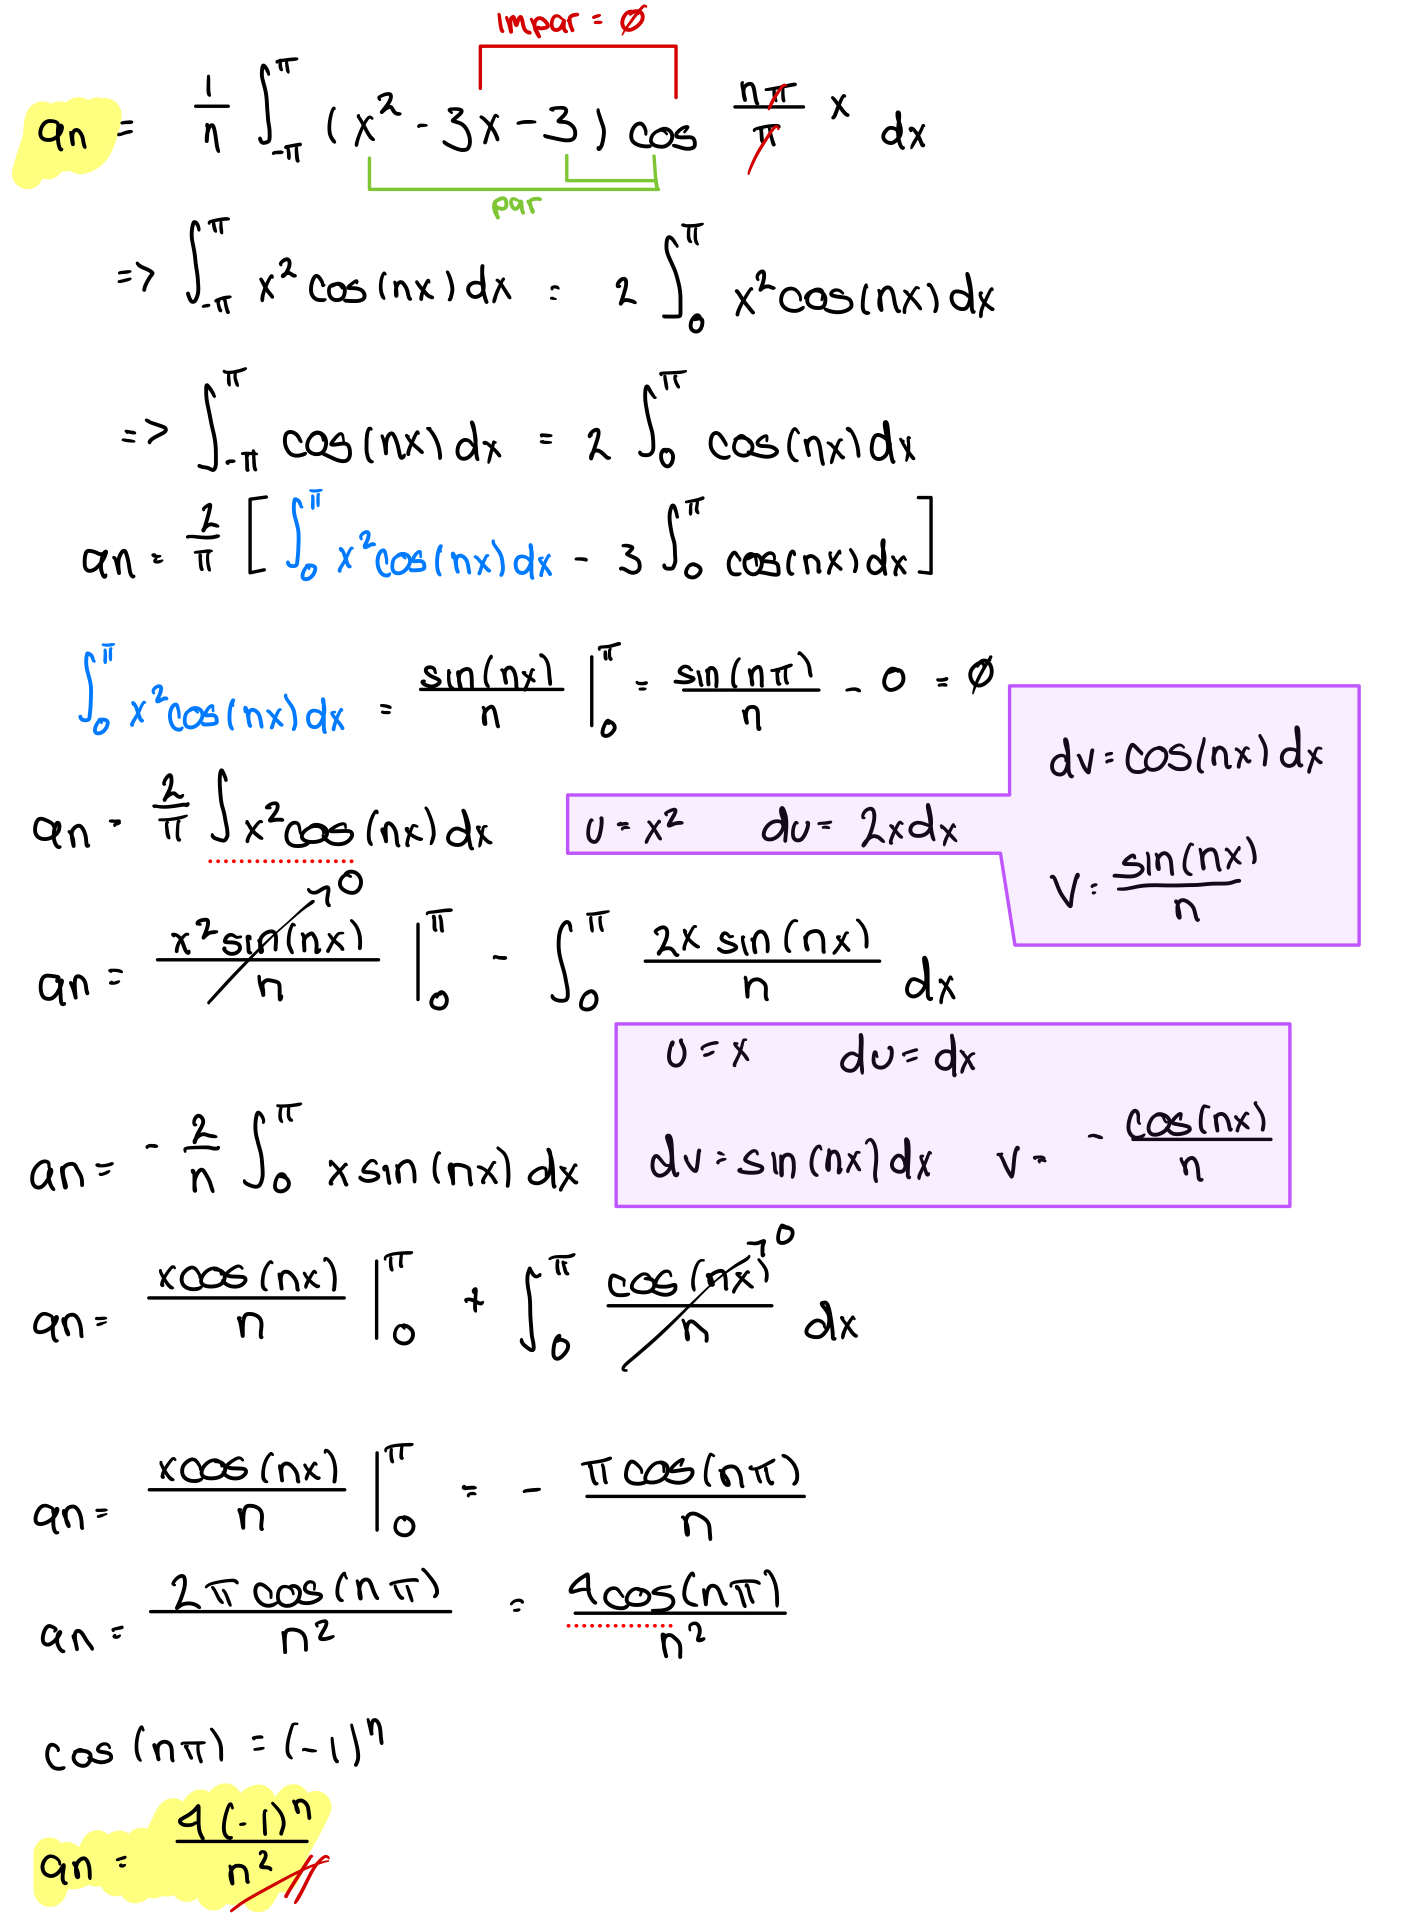
\includegraphics[width=\linewidth]{Figures/fourierManuel/an.jpeg}
        \caption[Cálculo de \(a_n\)]{Cálculo de \(a_n\), resuelto por Olguin Castillo.}
        \label{fig:figure-manuel-02}
    \end{figure}

\begin{figure}[H]
        \centering
        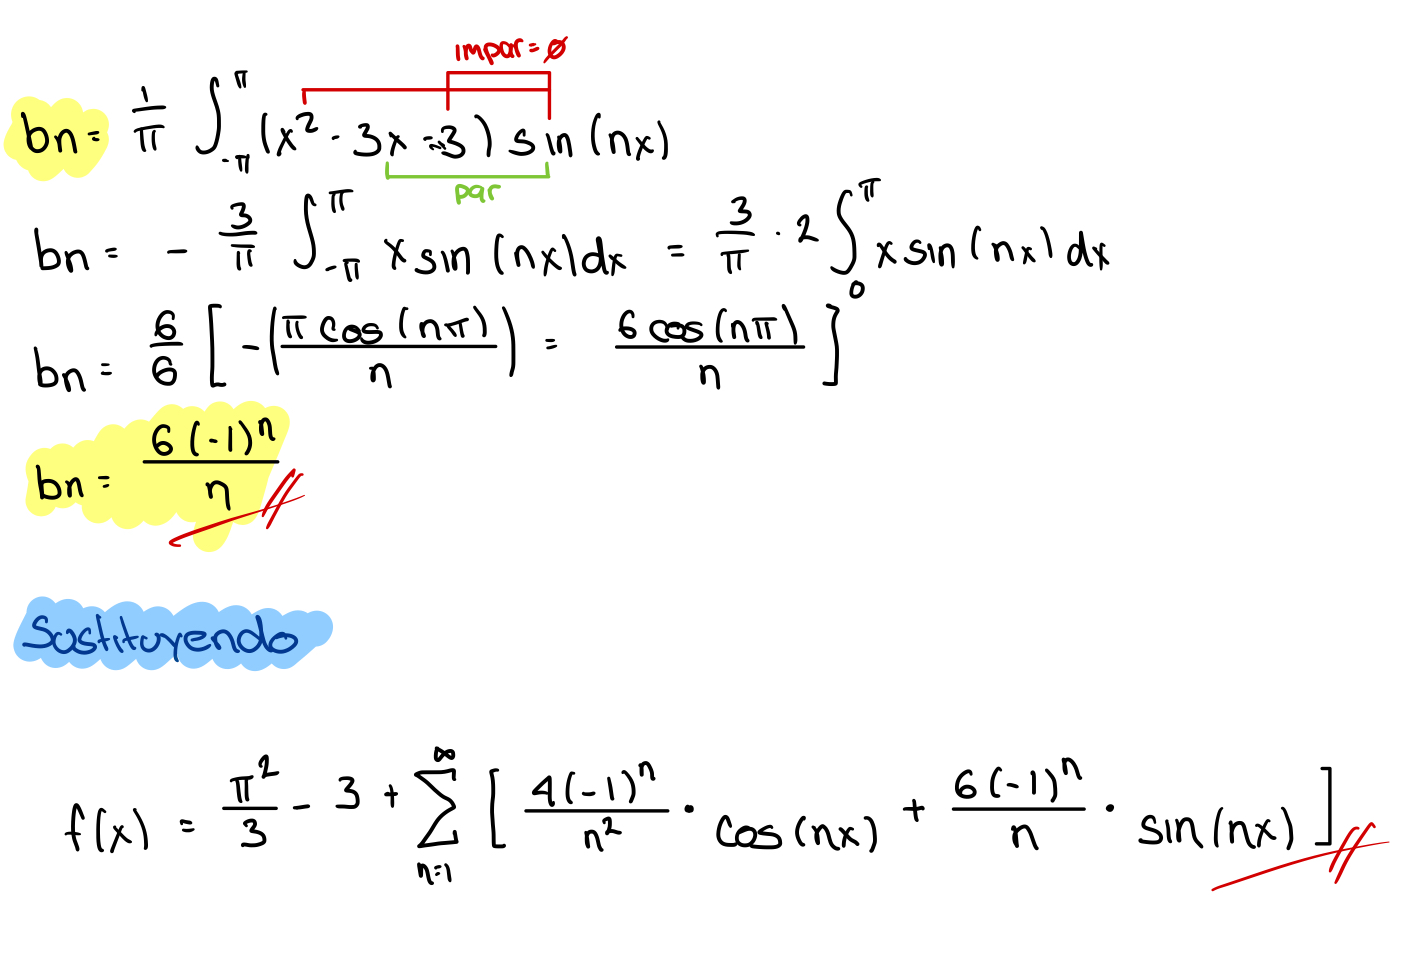
\includegraphics[width=\linewidth]{Figures/fourierManuel/bn.jpeg}
        \caption[Cálculo de \(b_n\)]{Cálculo de \(b_n\), resuelto por Olguin Castillo.}
        \label{fig:figure-manuel-03}
    \end{figure}

El método se basa en la expansión en series de Fourie usando simplificaciones algebraicas y las propiedades trigonométricas que permiten reducir la expresión final.



